
\usetikzlibrary{arrows}
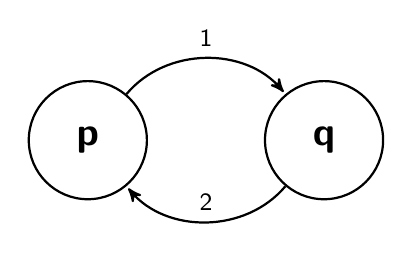
\begin{tikzpicture}[->,>=stealth',shorten >=1pt,auto,node distance=3cm,
  thick,main node/.style={circle,fill=white!10,draw,
  font=\sffamily\Large\bfseries,minimum size=15mm}]

  \node[main node] (p) {p};
  \node[main node] (q) [right of=p] {q};

  \path[every node/.style={font=\sffamily\small,
  		fill=white,inner sep=1pt}]
  	% Right-hand-side arrows rendered from top to bottom to
  	% achieve proper rendering of labels over arrows.
    (p) 
        edge [bend left=50] node[above=1mm] {1} (q)
    (q) 
        edge [bend left=50] node[above=1mm] {2} (p);
 
\end{tikzpicture}